\documentclass[12pt]{article}
\usepackage{braket}
\usepackage{physics}
\usepackage{graphicx}
\usepackage{times}
\usepackage[export]{adjustbox}
\usepackage{listings}
\usepackage{mathcomp}
\usepackage{hyperref}
\usepackage{bm,amsmath}
\usepackage{float}
\usepackage{indentfirst}
\usepackage{bigints}
\usepackage{listings}
\usepackage{color}
\hypersetup{
colorlinks=true,
linkcolor=blue,
filecolor=magenta,
urlcolor=cyan,
pdftitle={Overleaf Example},
pdfpagemode=FullScreen,
}
\definecolor{dkgreen}{rgb}{0,0.6,0}
\definecolor{gray}{rgb}{0.5,0.5,0.5}
\definecolor{mauve}{rgb}{0.58,0,0.82}
\lstset{frame=tb,
language=Python,
aboveskip=3mm,
belowskip=3mm,
stepnumber = 1,
showstringspaces=false,
columns=flexible,
basicstyle={\small\ttfamily},
numbers=left,
numberstyle=\color{gray},
keywordstyle=\color{blue},
commentstyle=\color{dkgreen},
stringstyle=\color{mauve},
breaklines=true,
breakatwhitespace=true,
tabsize=3
}
\numberwithin{equation}{section}

\title{Report On Performance of Simple Model and ParticleNet in Simple Particle Decay}
\author{Ting-Kai Hsu}
\date{\today}

\begin{document}
\maketitle
\tableofcontents
\section{Introduction}
In this report, we build out a simple neural network model in order to show ParticleNet isn't suitable for B-meson decay.
The architecture of the simple model would be
\begin{figure}[H]
    \centering
    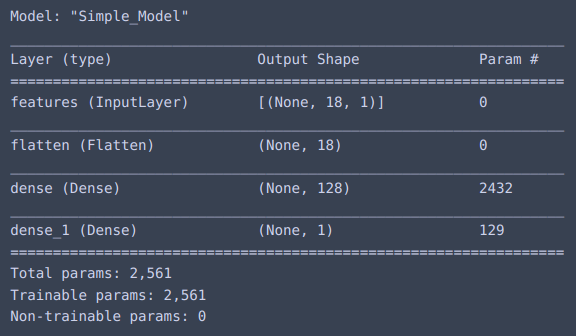
\includegraphics[width=0.75\linewidth]{Screenshot from 2024-06-22 00-15-47.png}
    \caption{Architecture of Simple Model}
    \label{1}
\end{figure}
\section{Decay Generator}
The generator of EvtGen can generator desired particles decay process.
Take B-meson decaying to PI+ and D0 for instance, the input size of simple model is $6\text{ (px,py,...) }*3\text{ (three particles)}$ without photon in consideration.
Total available events for training, validation, and test are listed,
\begin{table}[H]
    \centering
    \caption{Events in train.txt, val.txt, and test.txt}
        \begin{tabular}{|c|c|}
        \hline
        train & 55280\\
        \hline
        val & 6924\\
        \hline
        test & 7023\\
        \hline
        \end{tabular}
    \label{label}
\end{table}
\section{Results for 200 epochs}
The results of simple model and ParticleNet model are listed, respectively.
Note that the output is only mass prediction.
\begin{figure}[H]
    \centering
    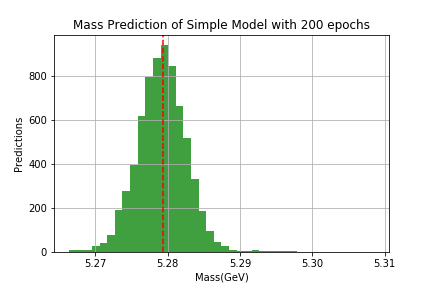
\includegraphics[width=0.75\linewidth]{SM200epochsw0Photon.png}
    \caption{Mass prediction of Simple Model with 200 epochs without photon}
    \label{2}
\end{figure}
\begin{figure}[H]
    \centering
    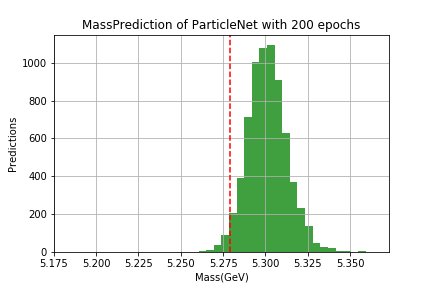
\includegraphics[width=0.75\linewidth]{PN200epochsw0Photon.png}
    \caption{Mass prediction of ParticleNet Model with 200 epochs without photon}
    \label{3}
\end{figure}
\section{Pros \& Cons}
ParticleNet model deals with jet tagging, and the model has made use of the spatial properties of jet.
However, B-meson decay doesn't have such spatial properties, so the performance of ParticleNet isn't good even in simple decay case.
The simple model can only deal with the case with fixed input, which makes it impractical in the physical process in reality.
\end{document}